\chapter{Harvey's algorithm}
\label{chap:harvey}

% \begin{enumerate}
%     \item Brief of the idea;
%     \item Pseudo-algorithm;
%     \item Corretude;
% \end{enumerate}
This chapter presents the probabilistic algorithm proposed by \citet{Harvey:Paper} that finds a perfect matching in general graphs with time complexity \(O(n^\omega)\).

\section{Algorithm}

The main bottleneck in the previous algorithm was the need to update the entire inverse matrix at each step. 
Harvey's algorithm addresses this limitation by employing a divide-and-conquer strategy combined with lazy updates. 
After each recursive step, only the necessary portions of the inverse matrix are updated.
As a result, Harvey's algorithm has a time complexity of \(O(n^\omega)\).

For a graph \(G\) and \(n = |V(G)|\),
the algorithm maintains two matrices, \(T\) and \(N\), that are initialized as
\begin{enumerate}
  \item \(T \coloneqq \) a Tutte matrix where the entries were randomly chosen, see \cref{sec:prob_tutte};
    \item \(N \coloneqq T^{-1}\).
\end{enumerate}
It relies on two recursive functions: \(\SC{DeleteEdgesCrossing}\) and \(\SC{DeleteEdgesWithin}\). 

\subsection{\(\SC{DivideInTwo}\)}
\(\SC{DivideInTwo(A)}\) is a function that divides a set \(A\) in two parts, \(R\) and \(S\), such that \(R \cup S = A\), \(R \cap S = \emptyset\) and \(|R| - |S| \leq 1\).
This function has time complexity \(O(n)\) and can be implemented through integer indexing the set.

\subsection{\(\SC{DeleteEdgesCrossing}\)}

$\SC{DeleteEdgesCrossing}(R, S)$: receives two disjoint sets of vertices \(R\) and \(S\) and 
deletes inessential edges with an end in \(R\) and the other in \(S\).
The following invariant must be preserved:
\begin{itemize}
  \item \(\SC{DeleteEdgesCrossing}(R, S)\): initially has \(N[R \cup S, R \cup S] = {T^{-1}}[R \cup S, R \cup S]\) and this property is restored after each call 
    of \(\SC{DeleteEdgesCrossing}(R_i, S_j)\).
\end{itemize}
To maintain this invariant the following updates are done. 
\begin{theorem}[Update 1\footnote{This update is different from the one in \citet{Harvey:Paper}.}]
\label{update:1}
    Let \(R, S\) be two disjoint sets of vertices such that \(|R| = |S| = 1\).
    Let \(N \coloneqq T^{-1}\), \(r \in R\) and \(s \in S\).
    If \(\{r, s\}\) is inessential, let \(\tilde{T}\) be the Tutte matrix of \(G\) without edge \(rs\), then one has
    \[
        \tilde{T}^{-1}_{r, s} = N_{r, s} / (1 + T_{r, s} N_{r, s})
    \]
    and
    \[
        \tilde{T}^{-1}_{s, r} = N_{s, r} / (1 + T_{r, s} N_{r, s}) = -\tilde{T}^{-1}_{r, s}.
    \]
\end{theorem}

\begin{proof}
  Let \(RS \coloneqq R \cup S\) and let \(\Delta \coloneqq \tilde{T}_{RS, RS} - T_{RS, RS}\).
By \cref{cor:update_cor}, one has:
\begin{align*}
  \tilde{T}^{-1}_{RS, RS} &= N_{RS, RS} - N_{RS, RS} (I + \Delta N_{RS, RS})^{-1} \Delta N_{RS, RS} & \\
                          &= N_{RS, RS} - N_{RS, RS} \begin{bmatrix} 1 + T_{r, s} N_{r, s} & 0 \\ 0 & 1 + T_{r, s} N_{r, s} \end{bmatrix}^{-1} \Delta N_{RS, RS} & \text{by \eqref{rank-two:eq}} \\
                     &= N_{RS, RS} - N_{RS, RS} \begin{bmatrix} 1 / (1 + T_{r, s} N_{r, s}) & 0 \\ 0 & 1 / (1 + T_{r, s} N_{r, s}) \end{bmatrix} \Delta N_{RS, RS} &\\
                     % &= N_{RS, RS} + N_{RS, RS} \begin{bmatrix} \frac{1}{1 + T_{r, s} N_{r, s}} & 0 \\ 0 & \frac{1}{1 + T_{r, s} N_{r, s}} \end{bmatrix} \begin{bmatrix} T_{r, s} N_{s, r} & 0 \\ 0 & T_{s, r} N_{r, s} \end{bmatrix} & \\
                     % &= N_{RS, RS} + N_{RS, RS} \begin{bmatrix} \frac{T_{r, s}N_{s, r}}{1 + T_{r, s} N_{r, s}} & 0 \\ 0 & \frac{T_{s, r}N_{r, s}}{1 + T_{r, s} N_{r, s}} \end{bmatrix} 
                     &= N_{RS, RS} + \begin{bmatrix} 0 & N_{r, s}T_{s, r}N_{r, s} / (1 + T_{r, s} N_{r, s}) \\ N_{s, r}T_{r, s}N_{s, r} /  (1 + T_{r, s} N_{r, s}) & 0 \end{bmatrix} & \\
                     % &= \begin{bmatrix} 0 & N_{r, s} + \frac{N_{r, s}T_{s, r}N_{r, s}}{1 + T_{r, s} N_{r, s}} \\ N_{s, r} + \frac{N_{s, r}T_{r, s}N_{s, r}}{1 + T_{r, s} N_{r, s}} & 0 \end{bmatrix} & \\
                     &= \begin{bmatrix} 0 & N_{r, s} / (1 + T_{r, s} N_{r, s}) \\ N_{s, r} / (1 + T_{r, s} N_{r, s}) & 0 \end{bmatrix}. & \qedhere
\end{align*}
\end{proof}

\begin{theorem}[Update 2]
\label{update:2}
    Let \(R, S\) be two disjoint set of vertices. Let \(\tilde{T}\) be \(T\) after removing some (possibly zero) edges from \(G\) with an end in \(R_i\) and another in \(S_j\).
    Let \(N := T^{-1}\) and \(\Delta := \tilde{T} - T\). Then
    \[
      {\tilde{T}}^{-1}[R \cup S, R \cup S] = N_{R \cup S, R \cup S} - N_{R \cup S, R_i \cup S_j}(I + \Delta N_{R_i \cup S_j, R_i \cup S_j})^{-1} \Delta N_{R_i \cup S_j, R \cup S}.
    \]
\end{theorem}

\begin{proof}
    Direct from \cref{cor:update_cor}. Update the whole matrix with \ref{cor:update_cor} and select only the desired submatrix.
\end{proof}

We have the following algorithm.

\newpage
\begin{programruledcaption}{Harvey's algorithm: \(\SC{DeleteEdgesCrossing}\)}
    \begin{lstlisting}[
      language={pseudocode},
      style=pseudocode,
      style=wider,
      functions={DeleteEdgesCrossing, RemoveEdge, DivideInTwo},
      specialidentifiers={},
    ]
        function DeleteEdgesCrossing(R, S) // R and S are \textbf{disjoint} sets of vertices.
            if $|R| = 0$ or $|S| = 0$ then return // There are no edges.

            if $|R| = 1$ and $|S| = 1$ then // There is at most \textbf{one} edge.
                Let $r$ in $R$
                Let $s$ in $S$
                if $T_{r, s} \neq 0$ \textbf{ and } $N_{r, s} \neq -1 / T_{r, s}$ then // \cref{cor:condition_edge_removal}.
                    $N_{r, s}$ := $N_{r, s} / (1 + T_{r, s} N_{r, s})$ // \cref{update:1}.
                    $N_{s, r}$ := $-N_{r, s}$
                    RemoveEdge($T, rs$)
                return

            $RS$ := $R \cup S$
            $R_1, R_2$ := DivideInTwo($R$)
            $S_1, S_2$ := DivideInTwo($S$)
            for i \textbf{in} {1, 2} do
                for j \textbf{in} {1, 2} do
                    $T', N'$ := $T, N$ // Save current T and N states
                    DeleteEdgesCrossing($R_i, S_j$)
                    $\Delta$ := $T[R_i \cup S_j, R_i \cup S_j] - {T'}[R_i \cup S_j, R_i \cup S_j]$
                    $N_{RS, RS}$ := $N_{RS, RS}' - {N_{RS, R_i \cup S_j}'} (I + \Delta {N_{R_i \cup S_j, R_i \cup S_j}'})^{-1} \Delta {N_{R_i \cup S_j, RS}'}$ // \cref{update:2}.
    \end{lstlisting}
\end{programruledcaption}

\subsubsection{Time complexity}
\noindent
Let \(f(r, s)\) be the running time for \(\SC{DeleteEdgesCrossing}(R, S)\) when \(|R| = r\) and \(|S| = s\).
Let \(n = r + s\). The base cases are \(O(1)\).
Otherwise, a line-by-line analysis:
\begin{enumerate}
    \item \textbf{Dividing in half (Lines 14 and 15)}: Takes \(O(n)\) time;
    \item \textbf{Saving the states (Line 18)}: Takes \(O(n^2)\) time;
    \item \textbf{Recursive call (Line 19)}: Recurrence is \(f(r/2, s/2)\);
    \item \textbf{Delta (Line 20)}: Matrix subtraction is \(O(n^2)\);
    \item \textbf{Update submatrix (Line 21)}: Takes \(O(n^\omega)\).
\end{enumerate}
Combining these steps, we have
\begin{align*}
    f(r, s) &= O(1) + O(1) + O(n^2) + 4(O(n^2) + f(r / 2, s / 2) + O(n^\omega))  \\
    &= 4O(n^2) + 4f(r / 2, s / 2) + 4O(n^\omega) \\
    &= 4f(r / 2, s / 2) + 4O(n^\omega).
\end{align*}
Now, applying the master theorem \cite[Theorem 4.1]{CLRS} for recursions, i.e. 
\[
  T(n) = aT(n/b) + f(n).
\]
In this case, \(T(n) = t(r, s)\), \(a = 4\), \(b = 2\) and \(f(n) = O(n^\omega)\), then if \(\omega > \log_{b}a = 2\) the complexity is dominated by \(O(n^\omega)\).
From \cref{matrix:time_complexity}, the best currently known matrix multiplication algorithm has \(\omega > 2\).
Thus, the complexity is dominated by \(O(n^\omega)\) and
\begin{equation}
  \label{alg:delcrossing}
  f(r, s) = 4f(r/2, s/2) + 4O(n^\omega) = 8O(n^\omega) = O(n^\omega). 
\end{equation}

\subsection{\(\SC{DeleteEdgesWithin}\)}

\(\SC{DeleteEdgesWithin}\): receives a set of vertices \(S\) and deletes inessential edges that have both ends in \(S\).
The following invariant must be preserved:
\begin{itemize}
  \item \(\SC{DeleteEdgesWithin}(S)\): initially has \(N[S, S] = T^{-1}[S, S]\) and this property is restored after each call of \(\SC{DeleteEdgesWithin}\)
    and \(\SC{DeleteEdgesCrossing}\).
\end{itemize}
To maintain this invariant the following update is done.
\begin{theorem}[Update 3]
\label{update:3}
    Let \(S \subseteq V_G\), let \(\tilde{T}\) be \(T\) after removing some (possibly zero) edges from \(G\) with both ends in \(S\).
    Then, let \(N \coloneqq T^{-1}\) and \(\Delta \coloneqq \tilde{T} - T\), one has
    \[
        {\tilde{T}}^{-1}_{S, S} = N_{S, S} - N_{S, S_i}(I + \Delta N_{S_i, S_i})^{-1} \Delta N_{S_i, S}.
    \]
\end{theorem}

\begin{proof}
    Direct from \cref{cor:update_cor}. Update the whole matrix using \ref{cor:update_cor} and select only the desired submatrix.
\end{proof}

We have the following algorithm.

\begin{programruledcaption}{Harvey's algorithm: \(\SC{DeleteEdgesWithin}\)}
    \begin{lstlisting}[
      language={pseudocode},
      style=pseudocode,
      style=wider,
      functions={DeleteEdgesCrossing, DeleteEdgesWithin, DivideInTwo},
      specialidentifiers={},
    ]
        function DeleteEdgesWithin(S)
            if |S| = 1 return

            $S_1, S_2$ := DivideInTwo($S, 2$)
            for i \textbf{in} {1, 2} do
                $T', N'$ := $T, N$ // Save current T and N states.
                DeleteEdgesWithin($S_i$)
                $\Delta$ := $T_{S_i, S_i} - {T_{S_i, S_i}'}$
                $N_{S, S}$ := $N' - {N_{S, S_i}'}(I + \Delta {N_{S_i, S_i}'})^{-1} \Delta {N_{S_i, S}'}$ // \cref{update:3}. 
            DeleteEdgesCrossing($S_1, S_2$)
    \end{lstlisting}
\end{programruledcaption}

\subsubsection{Time complexity}
\noindent
Let \(g(n)\) be the running time of \(\SC{DeleteEdgesWithin}(S)\) when \(|S| = n\).
The base case is direct.
Then, through a line-by-line analysis we have
\begin{enumerate}
  \item \textbf{DivideInTwo (Line 4)}: Takes \(O(n)\) times;
  \item \textbf{Saving the states (Line 6)}: Takes \(O(n^2)\) time;
  \item \textbf{Recursive call (Line 7)}: Takes \(g(n/2)\) time;
  \item \textbf{Delta (Line 8)}: Takes \(O(n^2)\);
  \item \textbf{Update 3 (Line 9)}: Takes \(O(n^\omega)\) time;
  \item \textbf{DeleteEdgesCrossing (Line 10)}: Takes \(f(n/2, n/2)\).
\end{enumerate}
Now, combining these steps:
\begin{align*}
    g(n) &= O(n) + 2 (2O(n^2) + g(n / 2) + O(n^\omega)) + f(n/2, n/2) &  \\
    &= O(n) + 2 (2O(n^2) + g(n / 2) + O(n^\omega)) + O(n^\omega) & \text{by \eqref{alg:delcrossing}} \\
    &= 2g(n / 2) + 3O(n^\omega).
\end{align*}
Similarly to \eqref{alg:delcrossing}, we have
\begin{equation}
\label{alg:delwithin}
  g(n) = 2g(n / 2) + 3O(n^\omega) = O(n^\omega).
\end{equation}

\subsection{\(\SC{PerfectMatching}\)}

\(\SC{PerfectMatching}\): Receives a graph \(G\) and finds a perfect matching, or returns \(\emptyset\) if one does not exist.
It creates a Tutte Matrix of \(G\) with random entries.
Note that calling \(\SC{DeleteEdgesWithin}(V(G))\) is equivalent to deleting every inessential edge from \(G\).
Thus, after this call, the graph only has essential edges, i.e. edges from the perfect matching. 
Consequently, there is the following implementation:

\begin{programruledcaption}{Harvey's algorithm: \(\SC{Perfect Matching}\)}
    \begin{lstlisting}[
      language={pseudocode},
      style=pseudocode,
      style=wider,
      functions={DeleteEdgesWithin},
      specialidentifiers={},
    ]
        function PerfectMatching(G)
            T := $\SC{TutteMatrix}(G)$
            if T \textbf{ is singular} then return $\emptyset$ // The graph has no perfect matching.
            N := $T^{-1}$
            DeleteEdgesWithin($V$)
            return $E(T)$
    \end{lstlisting}
\end{programruledcaption}

\subsubsection{Time complexity}
\noindent
Let \(T(n)\) be the running time of \(\SC{PerfectMatching(G)}\) when \(|V| = n\). 
A line-by-line comparison:
\begin{enumerate}
  \item \textbf{Building a TutteMatrix (Line 2)}: Takes \(O(n^2)\) time;
  \item \textbf{Checking if a matrix is singular (Line 3)}: Takes \(O(n^\omega)\) time;
  \item \textbf{Calculating a matrix inverse (Line 4)}: Takes \(O(n^\omega)\) time;
  \item \textbf{DeleteEdgesWithin (Line 5)}: From \eqref{alg:delwithin}, takes \(g(n) = O(n^\omega)\) time;
  \item \textbf{Returning the matching (Line 6)}: Takes \(O(n^2)\) time.
\end{enumerate}
Combining these steps, we have:
\begin{equation}
\label{alg:harvey_complexity}
    T(n) = O(n^2) + O(n^\omega) + O(n^\omega) + O(n^\omega) + O(n^2) = O(n^\omega).
\end{equation}

\subsubsection{Probability of failure}
\noindent
Let \(\delta\) be the probability of failure.
From \cref{lemma:schwartz-zippel}, deciding if an edge can be deleted fails with probability \(n / q\) where \(q\) is the size of the field. 
Since there are \(\binom{n}{2}\) edges, then 
\[
  \delta \leq \binom{n}{2} n / q < n^3 / q.
\]

\subsubsection{Correctness}
\noindent
To prove the algorithm's correctness, it suffices that for every edge \(uv \in E(G)\), when evaluating whether \(uv\) can be removed (using \cref{cor:condition_edge_removal}), one has \(N_{uv} = T^{-1}_{uv}\).
This equality is guaranteed by the invariants.
Since the updates ensure that the invariants are maintained throughout the algorithm, we can conclude that the edge removal decisions are correct.

\section{Experimental Analysis}
\label{Harvey:analysis}
\noindent
This section compares Harvey's algorithm with two perfect matching algorithms:
\begin{enumerate}
   \item The rank-two algorithm described in \cref{alg:rank-two};
   \item An implementation of the Edmonds-Blossom algorithm made by \citet{giovana:blossom}.
\end{enumerate}
\noindent
The naive algorithm was not compared due to its poor performance.
For reference, its performance is at least 100 times slower than the Rank-two algorithm in all cases.

\subsection{Methodology}

The implementations were evaluated using randomly generated graph instances created with the Erd\H{o}s-R\'enyi model. 
For each vertex count, 10 test graphs were generated, varying the probability of edge creation between each pair of vertices. 
Each test case number corresponded to a specific probability of edge creation between vertex pairs, as defined in \cref{tab:edge_perf}. 
A verification system was implemented to validate the correctness of all outputs.
\begin{table}[H]
  \centering
  \begin{tabular}{|c|c|}
    \hline
    Test number & Probability \\
    \hline
    1 & 0.10 \\
    2 & 0.20 \\
    3 & 0.25 \\
    4 & 0.50 \\
    5 & 0.50 \\
    6 & 0.50 \\
    7 & 0.75 \\
    8 & 0.75 \\
    9 & 0.75 \\
    10 & 1.00 \\
    \hline
  \end{tabular}
  \caption{Edge creation probability for each Perfect Matching test case number.}
  \label{tab:edge_perf}
\end{table}
Each of the 50 test cases was executed 50 times to account for machine performance variability, resulting in 2,500 total executions.

\subsubsection{Hardware specifications}

\noindent
The benchmark was executed in a computer with the following specifications:

\begin{center}
  \begin{tabular}{|c|c|}
    \hline
    CPU & Intel(R) Core(TM) i7-9750H \\
    \hline
    RAM & 32GB \\ 
    \hline
  \end{tabular}
\end{center}

\subsubsection{Algorithms tested}
The fast matrix multiplication algorithm was \textbf{not} implemented since its threshold is too high for application purposes.
Instead the trivial $O(n^3)$ algorithm was used, thus the tested algorithms have the following time complexities, where \(n\) is the number of vertices and \(m\) is the number of edges.
\begin{center}
  \begin{tabular}{|c|c|}
    \hline
    Algorithm & Time complexity \\
    \hline
    Rank-two algorithm & \(O(n^2m + n^3)\) \\
    Harvey's algorithm & \(O(n^3)\) \\
    Edmonds-Blossom algorithm & \(O(n^2m)\) \\
    \hline
  \end{tabular}
\end{center}

\subsection{Results}
\label{results:perfect_matching}

In \cref{fig:perf_matching} provides an overview of the algorithms performance throughout all test cases.
Even though the Edmonds-Blossom worst-case time complexity is theoretically worse than Harvey's algorithm, when \(m > n\) (which is true for all test cases with \(n = 200\)), 
it demonstrates superior performance in all cases.
Nonetheless, Harvey's algorithm outperforms the Rank-two algorithm for bigger graphs demonstrating a considerable improvement.
\begin{figure}[h]
  \centering
  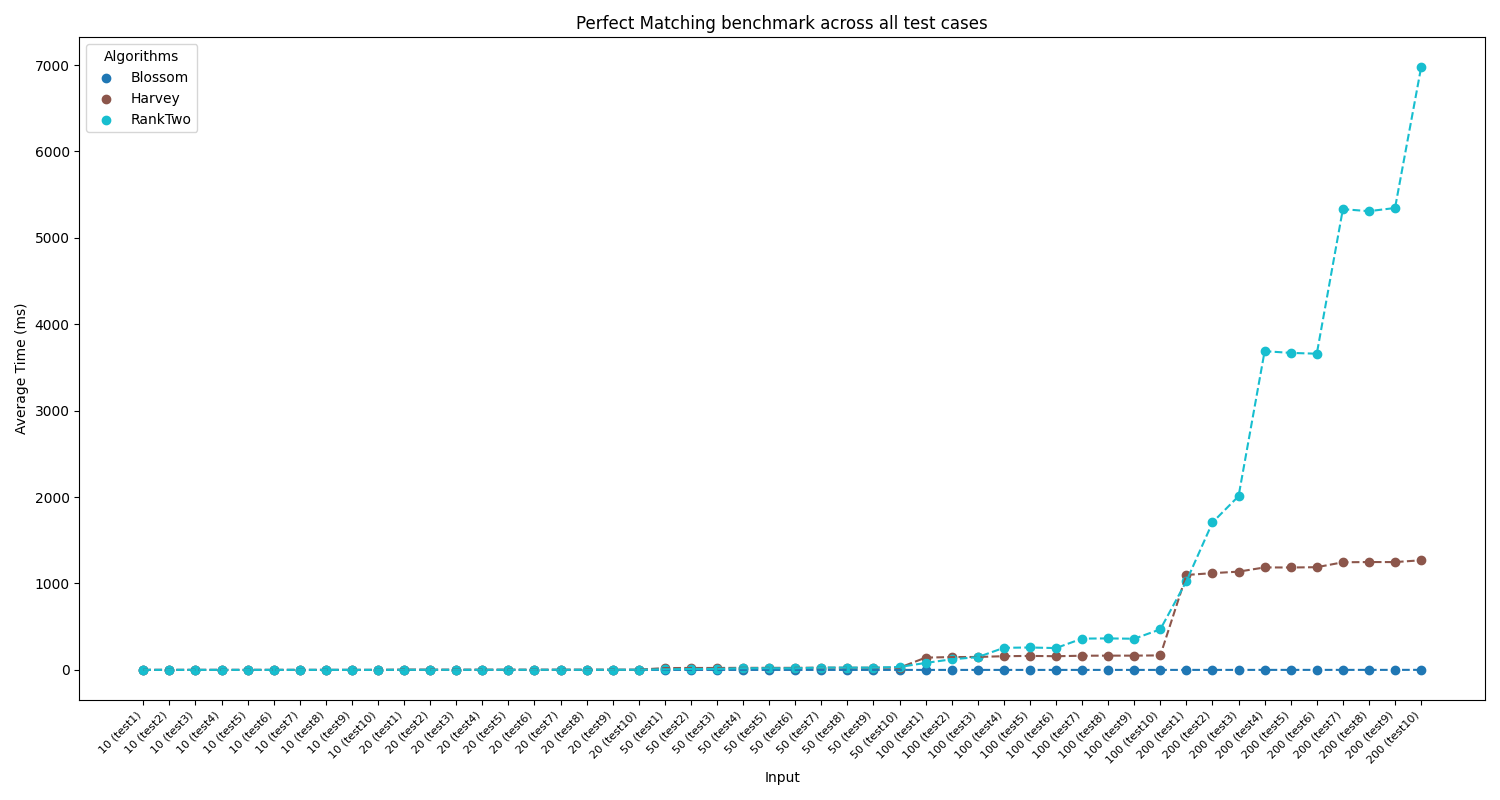
\includegraphics[width=15cm]{perfect_matching_plot.png}
  \caption{Perfect Matching benchmark with all test cases where the input number represents the number of vertices.}
  \label{fig:perf_matching}
\end{figure}

A more detailed case by case analysis follows. In \cref{fig:v10-20}, the Rank-two algorithm outperforms Harvey's algorithm with small \(n\), likely due to its lower constant factor. 

\begin{figure}[h]
  \centering
  \begin{subfigure}{.5\textwidth}
    \centering
    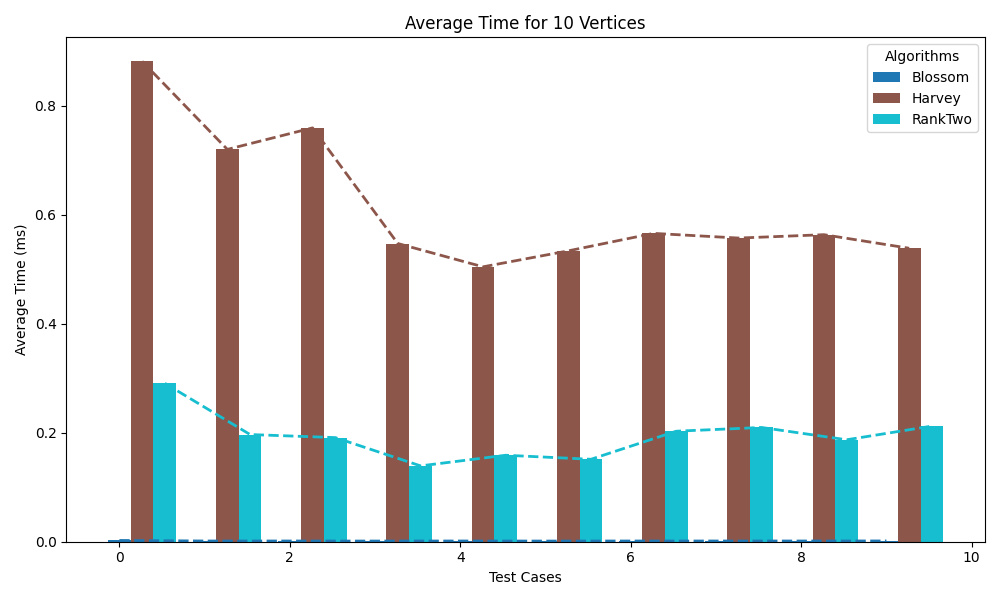
\includegraphics[width=\linewidth]{perfect_matching_10_vertices.png}
  \end{subfigure}%
  \begin{subfigure}{.5\textwidth}
    \centering
    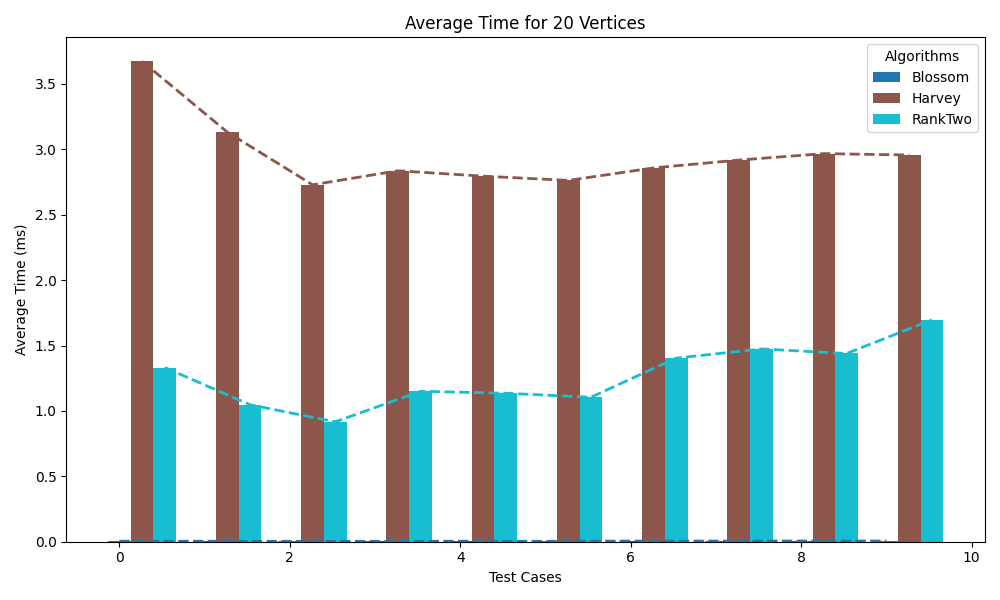
\includegraphics[width=\linewidth]{perfect_matching_20_vertices.png}
  \end{subfigure}
  \caption{Perfect Matching benchmark with 10 and 20 vertices.}
  \label{fig:v10-20}
\end{figure}

However, as the test sizes increase, Harvey's algorithm shows progressive improvement relative to the Rank-two algorithm. 
This trend becomes evident in \cref{fig:v50}, where the performance gap narrows significantly;
And, for the complete graph (e.g. the last test case), the Rank-two algorithm is outperformed by Harvey's algorithm.

\begin{figure}[h]
  \centering
  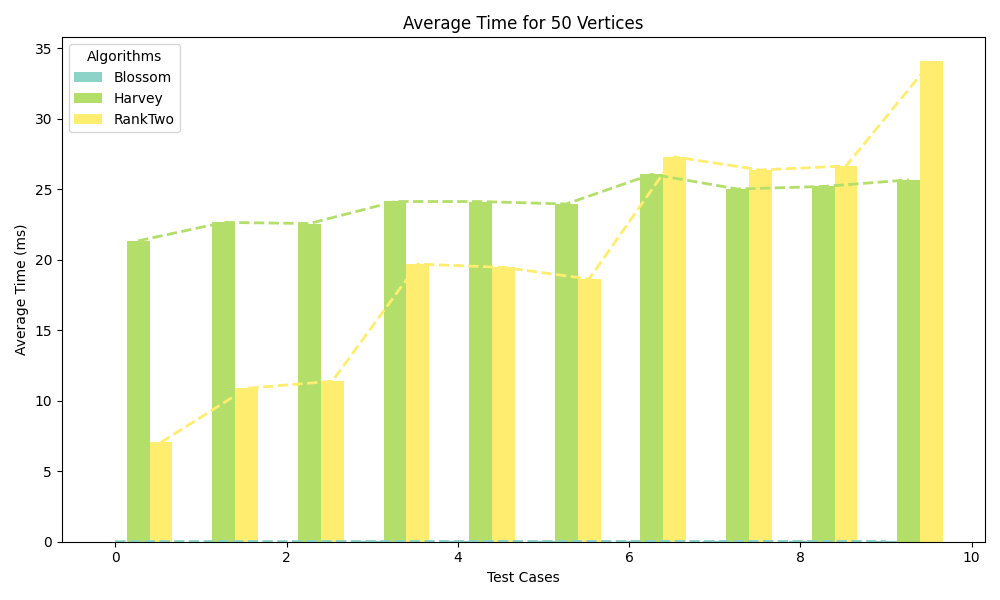
\includegraphics[width=12cm]{perfect_matching_50_vertices.png}
  \caption{Perfect Matching benchmark with 50 vertices.}
  \label{fig:v50}
\end{figure}

In \cref{fig:v100-200}, Harvey's algorithm ultimately achieves better overall performance than the Rank-two algorithm.
Notably the Rank-two algorithm exhibits significant performance variability, which can be attributed to its update frequency being directly tied to the number of edges removed from the graph. 
In contrast, Harvey's algorithm maintains consistent performance by executing a fixed number of updates, independent of the edge count. 
This behavior makes Harvey's algorithm more predictable in terms of execution time, particularly for larger graphs.

\begin{figure}[H]
  \centering
  \begin{subfigure}{.5\textwidth}
    \centering
    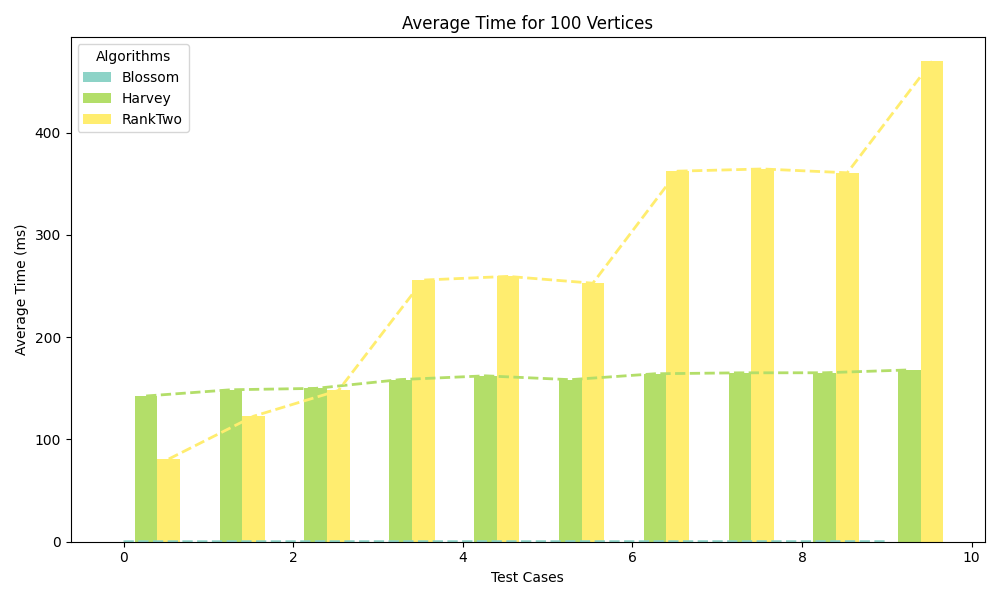
\includegraphics[width=\linewidth]{perfect_matching_100_vertices.png}
  \end{subfigure}%
  \begin{subfigure}{.5\textwidth}
    \centering
    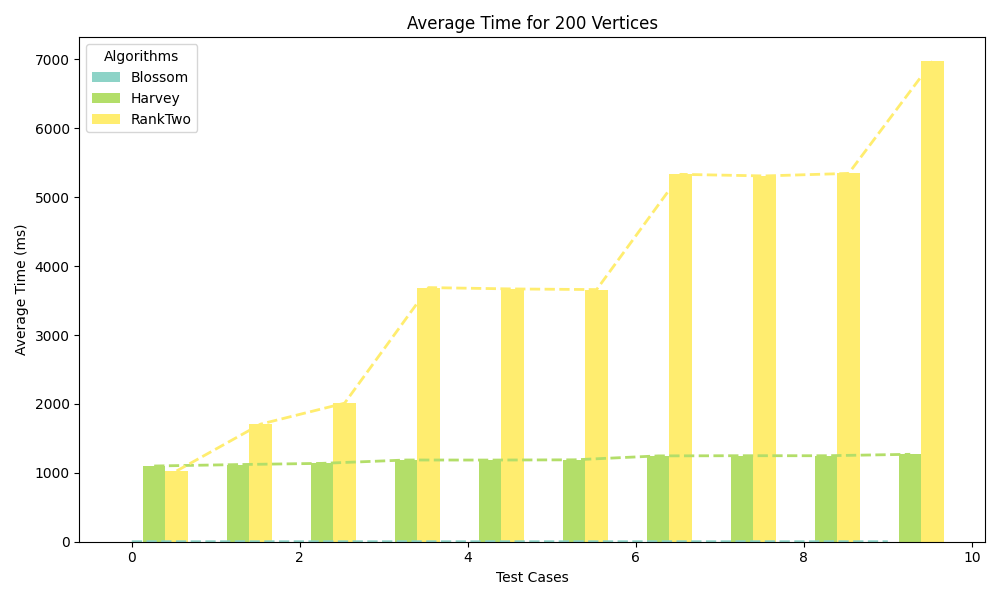
\includegraphics[width=\linewidth]{perfect_matching_200_vertices.png}
  \end{subfigure}
  \caption{Perfect Matching benchmark with 100 vertices and 200 vertices.}
  \label{fig:v100-200}
\end{figure}
